\chapter{Descripci\'on general de las herramientas num\'ericas}

El desarrollo y validaci\'on de modelos computacionales se encuentra intr\'insecamente vinculado a la existencia de una herramienta o plataforma num\'erica, capaz de ejecutar con precisi\'on, solidez y eficiencia aquellas t\'ecnicas bajo an\'alisis. 

Durante el comienzo del trabajo relacionado con esta tesis ya pod\'ian encontrarse herramientas desarrolladas dentro del \'ambito de LB con uso difundido en la industria e investigaci\'on, como PowerFlow \cite{noauthor_powerflow_nodate}, waLBerla \cite{noauthor_walberla_nodate}, PaLaBos \cite{latt_palabos_2020} u OpenLB \cite{noauthor_openlb_nodate}. Si bien estos productos ya contaban con varios a\~nos de desarrollo y podr\'ian haber sido elegidos para implementar los diferentes aspectos de este trabajo, a\'un exist\'ian caracter\'isticas primordiales que dificultaban su utilizaci\'on, y por lo tanto impulsaron la creaci\'on de una nueva herramienta. En particular, resulta crucial contar con un control estricto del flujo de informaci\'on dentro de la herramienta, sobre todo si se desea abordar la programaci\'on y verificaci\'on de nuevos modelos LB, destinados a resolver fen\'omenos f\'isicos no incluidos en los productos anteriores. Por otro lado, el dise\~no de un nuevo proyecto provee un mayor grado de flexibilidad y facilita la expansi\'on hacia nuevas \'areas, como la incorporaci\'on de soporte para nuevas arquitecturas de hardware.

En este contexto surge Phoenix, una herramienta desarrollada principalmente en C++ y destinada a la resoluci\'on de LBEs en sistemas distribuidos, como cl\'usters tradicionales de CPUs o unidades de procesamiento gr\'afico (CPU). Phoenix es un producto libre disponible en GitHub (\url{https://github.com/efogliatto/phoenix}), y que hasta el momento ha sido verificado para descarga, compilaci\'on y ejecuci\'on en sistemas Linux, en particular dentro de las distribuciones Debian/Ubuntu y Rocks. 
\nomenclature[A]{GPU}{\emph{Graphics Processing Units}}

El objetivo del presente cap\'itulo se reduce a incorporar una visi\'on global de los principales aspectos de dise\~no y funcionalidades de Phoenix. Una descripci\'on detallada de la API puede generarse de forma autom\'atica mediante las herramientas Doxygen y Sphinx, y el proyecto cuenta con numerosos casos de ejemplo para comprender el uso de las componentes del mismo.
\nomenclature[A]{API}{\emph{Application Programming Interface}}



\section{Estructura general del proyecto}

Phoenix fue dise\~nado como un conjunto de bibliotecas escritas en C++, destinadas a facilitar la programaci\'on de aplicaciones que permitan resolver LBEs, dentro de dominios computacionales con geometr\'ia arbitraria. 

La utilizaci\'on de clases en C++ permite incorporar diversas capas de abstracci\'on en el dise\~no general. De esta manera, durante el desarrollo de nuevas aplicaciones es posible manipular campos escalares, vectoriales o funciones de distribuci\'on sin necesidad de conocer la implementaci\'on asociada a la inicializaci\'on, lectura, escritura, o distribuci\'on entre procesos. Esta caracter\'istica fundamental aporta, en principio, un elevado nivel de extensibilidad al proyecto.

Las etapas de construcci\'on, compilaci\'on y prueba de Phoenix son gestionadas a trav\'es de la familia de herramientas conocida como CMake \cite{noauthor_cmake_nodate}. Estas utilidades se basan en el uso de archivos de configuraci\'on independientes de la plataforma o compilador, y permiten generar archivos Makefile nativos y \emph{workspaces} que son utilizados posteriormente por el compilador de elecci\'on. Entre otros aspectos, esto permite llevar a cabo una organizaci\'on sencilla del c\'odigo fuente, usando una estructura de directorios accesible para el programador. Por otro lado, el uso de CMake facilita la detecci\'on de bibliotecas y dependencias del sistema operativo, eligiendo adecuadamente las opciones de compilaci\'on en funci\'on de este entorno.

El \'arbol general del proyecto puede observarse en la \fig{fig:phoenix_struct}, donde se muestra el contenido del directorio principal, el subdirectorio \texttt{src} con el c\'odigo fuente, y un ejemplo con la ubicaci\'on de las declaraciones de clases usadas para la contrucci\'on de las ecuaciones de energ\'ia presentadas en los cap\'itulos anteriores. 

\begin{figure}[ht]
	\centering
\begin{forest}
      for tree={
        font=\ttfamily,
        grow'=0,
        child anchor=west,
        parent anchor=south,
        anchor=west,
        calign=first,
        inner xsep=7pt,
        edge path={
          \noexpand\path [draw, \forestoption{edge}]
          (!u.south west) +(7.5pt,0) |- (.child anchor) pic {folder} \forestoption{edge label};
        },
        % style for your file node 
        file/.style={edge path={\noexpand\path [draw, \forestoption{edge}]
          (!u.south west) +(7.5pt,0) |- (.child anchor) \forestoption{edge label};},
          inner xsep=2pt,font=\small\ttfamily
                     },
        before typesetting nodes={
          if n=1
            {insert before={[,phantom]}}
            {}
        },
        fit=band,
        before computing xy={l=15pt},
      }  
    [Phoenix
      [CMakeLists.txt,file
      ]    
      [bin
      ]
      [build
      ]     
      [cmake
      ]     
      [docs
      ]    
      [examples
      ]        
      [include
      ]       
      [lib
      ]   
      [src
        [CMakeLists.txt,file
        ]
        [algebra
        ]
        [applications
        ]
        [fdEquations
        ]      
        [forces
        ]
        [geometry
        ]
        [heatSources
        ]
        [IO
        ]                                
        [latticeFields
        ]        
        [latticeModel
        ]
        [lbEquations
	        [lbEquation.C,file
	        ]
%	        [lbEquation.H,file
%	        ]
        	    [energy
        	        [myMRTEq.C,file
        	        ]
%        	        [myMRTEq.H,file
%        	        ]        	        
        	    ]
        ]
        [mesh
        ]
        [relaxModel
        ]
        [simulation
        ]
        [tools
        ]
      ]   
      [tests
      ]             
    ]
 \end{forest}	
	\caption{Estructura de directorios de Phoenix}
	\label{fig:phoenix_struct}
\end{figure}
\FloatBarrier	

El cuerpo principal incluye los siguientes directorios:

\begin{itemize}
	\item \texttt{bin}: Directorio con ejecutables de aplicaciones y utilidades.
	\item \texttt{build}: Directorio de configuraci\'on y compilaci\'on.
	\item \texttt{cmake}: Opciones de configuraci\'on adicionales para CMake.
	\item \texttt{docs}: Contiene el resultado de la documentaci\'on autom\'atica generada por Doxygen y Sphinx.
	\item \texttt{examples}: Casos de ejemplo completos para demostrar el uso de Phoenix.
	\item \texttt{include}: Directorio con links simb\'olicos a todos las cabeceras (\texttt{.H})
	\item \texttt{lib}: Directorio con las bibliotecas compiladas, por el momento, del tipo compartidas (\emph{shared}).
	\item \texttt{src}: Directorio con el c\'odigo fuente, es decir, declaraciones de clases, utilidades y aplicaciones.
	\item \texttt{tests}: Casos de prueba dise\~nados para verificar el correcto funcionamiento de las diversas clases.
	
\end{itemize}


El contenido del directorio \texttt{src} se encuentra organizado para facilitar la construcci\'on de bibliotecas a partir de la funcionalidad de las diferentes clases. De esta manera, el conocimiento de su estructura aporta una descripci\'on general de las capacidades y alcances de la herramienta.

\begin{itemize}
	\item \texttt{algebra}: Manipulaci\'on de matrices espec\'ificas para los operadores de colisi\'on MRT.
	\item \texttt{applications}: Utilidades y aplicaciones, como los simuladores de flujo multif\'asico, malladores, generadores de condiciones iniciales, etc. Esta versi\'on tiene desarrollado los resolutores para modelos pseudopotencial isot\'ermico (\texttt{multiPhasePP}) y con transferencia de calor (\texttt{multiPhasePPHT}).
	\item \texttt{fdEquations}: Clases para resoluci\'on de EDPs mediante el m\'etodo de diferencias finitas.
	\item \texttt{forces}: Manipulaci\'on de distintos tipos de fuerza para ser incluidos en las LBE, como fuerza volum\'etrica, de interacci\'on y adhesi\'on.
	\item \texttt{geometry}: Elementos geom\'etricos b\'asicos, usados principalmente en la construcci\'on de campos iniciales y en la aplicaci\'on de condiciones de contorno.
	\item \texttt{heatSources}: Elementos de fuente para las ecuaciones de energ\'ia.
	\item \texttt{IO}: Clases para el manejo de entrada y salida de datos, como lectura y escritura de campos.
	\item \texttt{latticeFields}: Clases para la manipulaci\'on en alto nivel de variables escalares (\texttt{scalarField}), vectoriales (\texttt{vectorField}) y \fdp{} (\texttt{pdfField})
	\item \texttt{latticeModel}: Modelos de grilla (DqQq).
	\item \texttt{lbEquations}: Manipulaci\'on de ecuaciones LBE. Condiciones de contorno.
	\item \texttt{mesh}: Clases para la interpretaci\'on del mallado espacial. Incluye los aspectos principales de paralelizaci\'on (descomposici\'on del dominio), y constituyen la base para construir los campos de \texttt{latticeFields}.
	\item \texttt{relaxModel}: Diferentes modelos para los factores de relajaci\'on. Por ejemplo, consideraci\'on de variaci\'on espacial o dependencia con el valor de ciertos campos macrosc\'opicos en cada nodo.
	\item \texttt{simulation}: Clases para control de una simulaci\'on. Tiempo de comienzo y finalizaci\'on, intervalo de escritura o formato de entrada/salida.
	\item \texttt{tools}: Herramientas adicionales para complementar el uso de Phoenix. Esta versi\'on incluye m\'odulos de Python para construir mallas LB en SALOME \cite{noauthor_salome_nodate}.
\end{itemize}




\section{Malla}

\subsection{Generaci\'on de malla}

La malla o grilla utilizada por Phoenix consiste en un conjunto de nodos en un espacio tridimensional, distribuidos en un arreglo con espaciado uniforme en cada direcci\'on principal ($x$,$y$,$z$). Cada nodo se caracteriza por un conjunto de coordenadas espaciales, y por un conjunto de \'indices que indican cu\'ales son los nodos vecinos. En particular, esta representaci\'on de conectividad se realiza en base a un conjunto de velocidades de grilla D$d$Q$q$, de modo que cada nodo tiene $q$ vecinos y cada uno est\'a vinculado a una velocidad de grilla.

Phoenix cuenta con dos aplicaciones para generar mallas r\'apidamente en dominios rectangulares o prism\'aticos, llamadas \texttt{latticeBox2D} y \texttt{latticeBox3D}. Estas herramientas permiten seleccionar el modelo de velocidades de grilla desde un archivo de configuraci\'on, as\'i como las dimensiones principales (en unidades de grilla) necesarias en cada direcci\'on.

Esta representaci\'on mediante nodos y vecinos conectados permite expandir trivialmente el tipo de geometr\'ias a representar. En este caso, no es necesario restringirse a rect\'angulos o prismas, sino que pueden adaptarse dominios con bordes curvos mediante una superficie escalonada, como se ejemplifica en la \fig{fig:bunny}. Para ello, se cuenta con la herramienta nativa \texttt{cartesianMesh}, que construye una grilla regular delimitada por una superficie en formato STL mediante el uso de la biblioteca de geometr\'ia computacional CGAL \cite{noauthor_cgal_nodate}. Por otro lado, el m\'odulo \texttt{salomesh} permite construir una malla con la informaci\'on necesaria directamente dentro de SALOME.

\begin{figure}[ht]
	\centering
	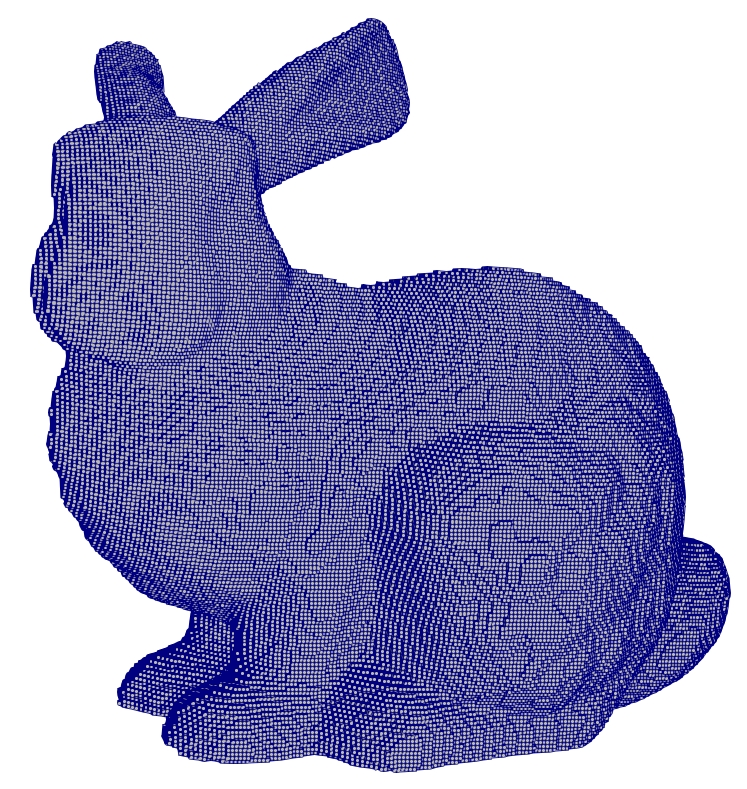
\includegraphics[width=0.6\textwidth]{Phoenix/bunny}
	\caption{Ejemplo de malla escalonada generada con \texttt{cantesianMesh}.}
	\label{fig:bunny}
\end{figure}

Los nodos que se encuentran en la frontera son aquellos que tienen incompleta la lista de vecinos. \'Estos pueden agruparse en conjuntos sobre los que podr\'an aplicarse diferentes condiciones de contorno, elegibles en tiempo de ejecuci\'on.


\subsection{Paralelizaci\'on}

Phoenix fue dise\~nado para soportar, de manera nativa, la utilizaci\'on de mallas obtenidas a partir de algoritmos de descomposici\'on de dominio. Como se ejemplifica en la \fig{fig:patch_based}, la grilla subyacente se interpreta a partir de un dise\~no \emph{patch-based}, donde la grilla principal est\'a compuesta por diferentes bloques. Cada bloque posee un conjunto de nodos propios, y contiene informaci\'on de nodos conectados que pertenecen a bloques vecinos (nodos fantasma o \emph{ghost}). De esta manera, los campos y ecuaciones definidos en cada bloque pueden manipularse de manera independiente por diferentes procesos o nodos computacionales, y se efect\'ua la sincronizaci\'on de los nodos fantasma mediante la implementaci\'on de funciones de OpenMPI. 

\begin{figure}[ht]
	\centering
	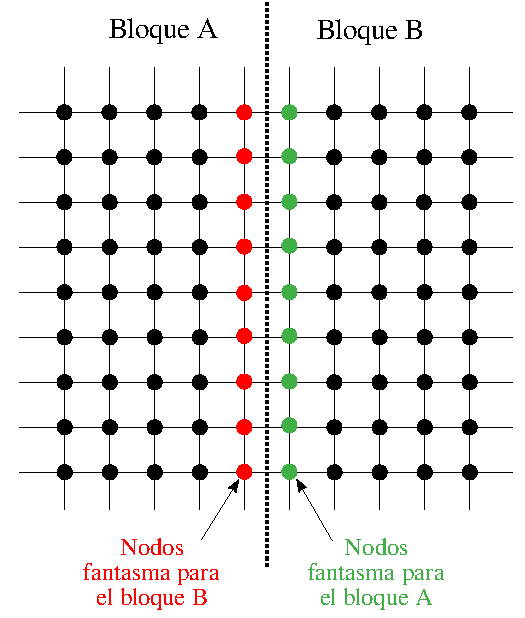
\includegraphics[width=0.75\textwidth]{Phoenix/grid_ghosts}
	\caption{Interpretaci\'on de malla con criterio \emph{patch-based}.}
	\label{fig:patch_based}
\end{figure}

Phoenix incorpora la utilidad \texttt{latticeMeshPartition} para descomponer una malla (generada por herramientas propias o externas) mediante diferentes algoritmos, como divisi\'on equitativa de nodos o mediante la biblioteca METIS.

El soporte de sistemas distribuidos fue desarrollado espec\'ificamente para este proyecto y no requiere de otras bibliotecas, como la popular PETSc. Las caracter\'isticas intr\'insecas de un algoritmo LB hacen que sea posible implementar, sin un esfuerzo de programaci\'on excesivo, una estructura funcional, robusta y eficiente sin necesidad de incorporar aquella sobrecarga introducida por una biblioteca m\'as general. 

En la \fig{fig:speedup_cpu} se muestra el resultado de una prueba de escalabilidad, definido a trav\'es de \emph{Speed Up}:
\begin{equation}
	Speed\,Up = t_r / t,
\end{equation}
donde $t_r$ es un tiempo de ejecuci\'on de referencia, como el correspondiente a 1 n\'ucleo o nodo (20 n\'ucleos), y $t$ el tiempo de c\'alculo actual. Esta prueba fue implementada en el cluster del Departamento de Mec\'anica Computacional (MECOM), con nodos Xeon Phi \red{data}. En la misma se ejecut\'o el problema de construcci\'on de Maxwell isot\'ermico en 3 dimensiones, sobre un dominio c\'ubico con $256^3$ nodos. Como se observa en la figura, el incremento en la cantidad de nodos utilizados produce un rendimiento similar al te\'orico si se utiliza la red de conexi\'on Infiniband, e incluyo muestra un comportamiento altamente satisfactorio durante el empleo de la red Gigabit-Ethernet.

\begin{figure}[ht]
	\centering
	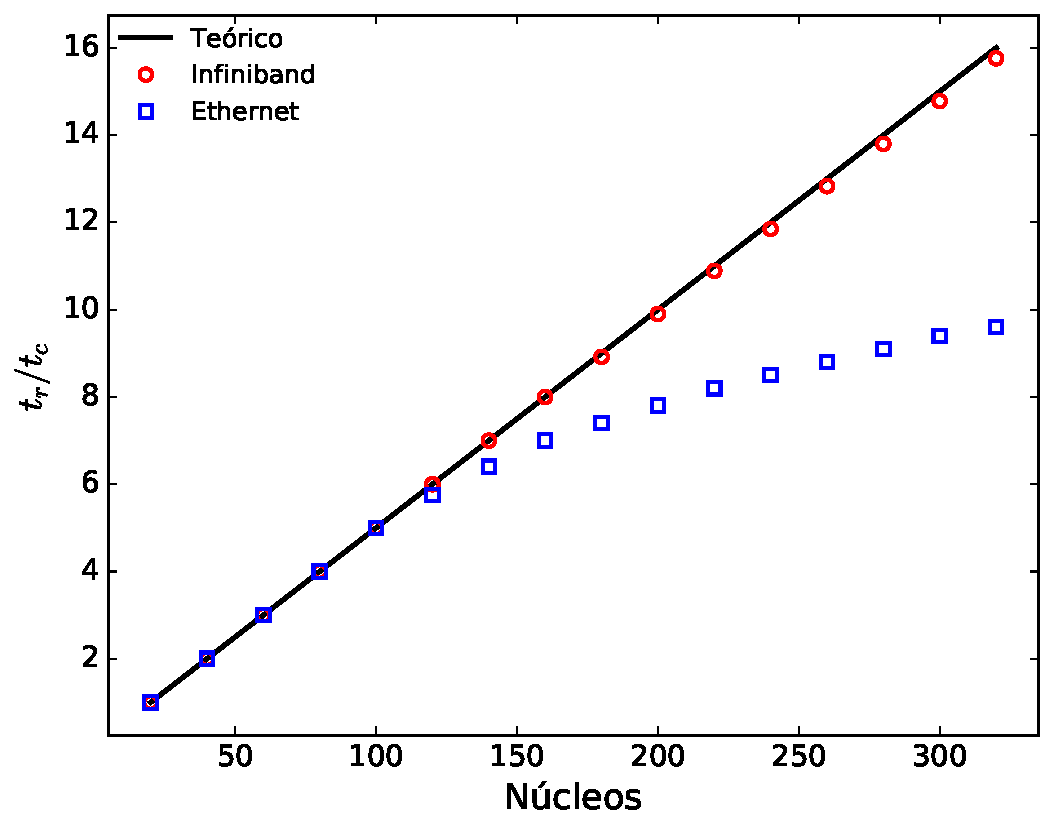
\includegraphics[width=0.75\textwidth]{Phoenix/SpeedUp}
	\caption{Prueba de \emph{Speed Up} para la aplicaci\'on de flujo multif\'asico isot\'ermico.}
	\label{fig:speedup_cpu}
\end{figure}




\section{Campos y variables}

Las variables f\'isicas como densidad, velocidad, temperatura o funciones de distribuci\'on son representadas mediante clases apropiadas. Las mismas se encuentran construidas sobre las mallas descriptas previamente, de modo que adquieren autom\'aticamente el car\'acter de entidades distribuidas. De esta manera, pueden inspeccionarse dentro de cada proceso s\'olo sincronizan la informaci\'on asociada a los nodos fantasmas.

Las clases \texttt{scalarField}, \texttt{vectorField} y \texttt{pdfField} contienen m\'etodos que permiten su lectura y escritura en formato ENSIGHT GOLD. Esta representaci\'on ofrece un buen compromiso entre espacio de almacenamiento y velocidad de lectura/escritura, ya que admite una estructura de bloques (similares a los bloques de cada proceso) en formato binario. Por otro lado, este formato es admisible en herramientas de post-procesamiento como ParaView.

Todos los campos pueden inicializarse, antes de cada simulaci\'on, mediante la herramienta \texttt{setInitialFields}. La misma transforma instrucciones de un archivo de configuraci\'on en una distribuci\'on espacial para el campo indicado. De esta manera es posible construir una matriz de cierta densidad con una burbuja esf\'erica en su interior, o incorporar un perfil lineal de temperatura dentro de una cavidad.



\section{Ecuaciones}

La resoluci\'on de una (o varias) LBE puede llevarse a cabo siguiendo un algoritmo general, similar a la interpretaci\'on est\'andar de una ecuaci\'on de LB. Como se muestra en el extracto de c\'odigo de la \fig{fig:eq_handler}, las clases \emph{equation handler} permiten implementar un algoritmo abstracto de LB: cada LBE tiene asociados campos o variables, y hay que efectuar una colisi\'on, advecci\'on, aplicaci\'on de condiciones de contorno y actualizaci\'on de variables macrosc\'opicas.

\begin{figure}[ht]
	\centering
	\begin{lstlisting}[language=C++]

	// Distribution function		
	pdfField f( mesh, Time, "f", IO::MUST_READ, IO::MUST_WRITE );	
	
	// Equation handler	
	pseudoPotEqHandler NS("Navier-Stokes", mesh, Time, f, rho, U, T);
	
	// Solve Navier-Stokes equation
	NS.collision();
	NS.streaming();
	NS.updateBoundaries();
	f.sync();
	
	// Update macroscopic fields
	NS.updateMacroDensity();
	NS.updateMacroVelocity();
	\end{lstlisting}
	\caption{Extracto de c\'odigo que ejemplifica el uso de un \emph{equation handler}}
	\label{fig:eq_handler}
\end{figure}

Las ecuaciones son generadas a partir de la clase abstracta \texttt{lbEquation}, como se muestra en el diagrama de herencia de la \fig{fig:lbeq_her}. Cada una de las clases heredadas est\'a asociada a un modelo f\'isico concreto, y contiene una definici\'on espec\'ifica del proceso de colisi\'on y c\'alculo de momentos macrosc\'opicos.

El uso de ecuaciones espec\'ificas dentro de cada aplicaci\'on se realiza en tiempo de ejecuci\'on, es decir, eligiendo el modelo f\'isico mediante la lectura de un archivo de configuraci\'on. Esta caracter\'istica es posible gracias a la aplicaci\'on extensiva del patr\'on de dise\~no conocido como f\'abrica o \emph{factory pattern}.

\begin{figure}[ht]
	\centering
	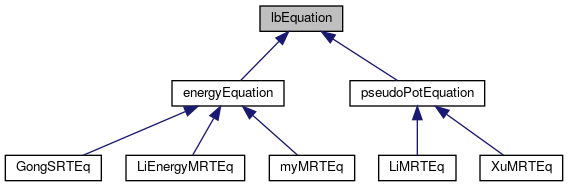
\includegraphics[width=0.75\textwidth]{Phoenix/classlbEquation__inherit__graph}
	\caption{Diagrama de herencia de la clase \texttt{lbEquation}.}
	\label{fig:lbeq_her}
\end{figure}

La utilizaci\'on del patr\'on de f\'abrica resulta \'util para seleccionar instancias de clases en tiempo de ejecuci\'on, lo que permite la selecci\'on no s\'olo de los modelos de LBE sino tambi\'en de las condiciones de contorno. En la \fig{fig:energy_bnd} se muestra el diagrama de herencia de la clase abstracta \texttt{energyBndCond}, cuyos hijos pueden construirse mediante la f\'abrica \texttt{energyBndCreator}. En la pr\'actica, este dise\~no permite resolver una LBE de energ\'ia y seleccionar, en tiempo de ejecuci\'on, la aplicaci\'on de una condici\'on de contorno de temperatura fija, flujo de calor, \emph{outflow}, temperatura o flujo de calor con \emph{spots}, etc. Con este mismo criterio tambi\'en es posible seleccionar esquemas de fuerza de interacci\'on, tipos de fuerza de adhesi\'on, ecuaciones de estado o modelos para factores de relajaci\'on.

\begin{figure}[ht]
	\centering
	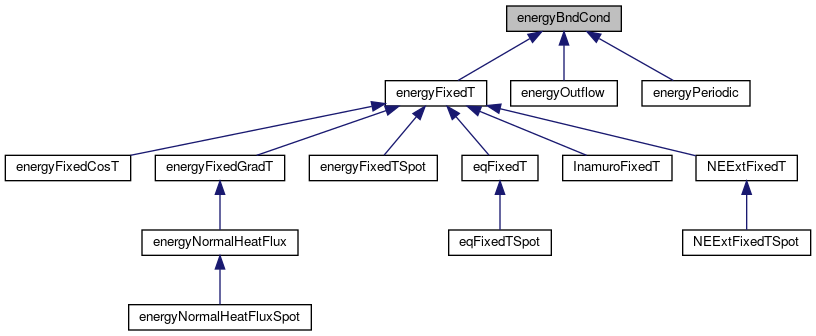
\includegraphics[width=0.75\textwidth]{Phoenix/classenergyBndCond__inherit__graph}
	\caption{Diagrama de herencia de la clase \texttt{lbEquation}.}
	\label{fig:energy_bnd}
\end{figure}



\section{Implementaci\'on en CUDA}

Las caracter\'isticas distintivas de los algoritmos LB los convierten en candidatos ideales para su implementaci\'on en sistemas de procesamiento masivo en paralelo. En esta l\'inea, no s\'olo es posible desarrollar proyectos para el c\'alculo en m\'ultiples CPUs, sino que tambi\'en puede aprovecharse directamente el paralelismo nativo de las CPU.

Estas ventajas motivaron el desarrollo del proyecto LBCUDA (\url{https://github.com/efogliatto/LBCUDA}), una implementaci\'on en CUDA del modelo multif\'asico con transferencia de calor descripto en el \chap{chap:modelo2D}, que deriv\'o en el desarrollo de una Tesis de Proyecto Integrador en el Instituto Balseiro \cite{coronel_implementacion_2020}. Si bien este proyecto no es parte de Phoenix, su estructura y ciertas funciones fueron heredadas directamente del mismo. LBCUDA implementa los m\'etodos de algunas clases heredadas de \texttt{lbEquations} como funciones o \emph{kernels} de CUDA, permitiendo su ejecuci\'on en unidades de procesamiento gr\'afico.

La API de LBCUDA se encuentra documentada con Doxygen dentro del mismo proyecto y el proceso de desarrollo y validaci\'on puede encontrarse en \cite{coronel_implementacion_2020}, por lo no se incluir\'an estos detalles en este cap\'itulo. Sin embargo, resulta interesante destacar ciertos resultados del an\'alisis de eficiencia del proyecto, desarrollados en base a la resoluci\'on del problema de construcci\'on de Maxwell isot\'ermico. Como se observa en las \figs{fig:lbcuda_760_simple}{fig:lbcuda_760_doble}, la resoluci\'on de este problema en una GPU NVIDIA GeForce GTX 760 es 18 veces m\'as r\'apida en simple precisi\'on que la versi\'on equivalente en C, resuelta en un procesador Intel Core i7-3770. Para doble precisi\'on, esta diferencia es cercana a 12 veces. Por otro lado, como se destaca en \cite{coronel_implementacion_2020}, la aceleraci\'on alcanzada por una GPU NVIDIA GeForce GTX 970 alcanza las 24 veces respecto a la versi\'on en CPU. Estos resultados muestran el gran potencial de la t\'ecnica, y la importancia de migrar hacia sistemas basados en GPUs.

\begin{figure}[ht]
	\centering
	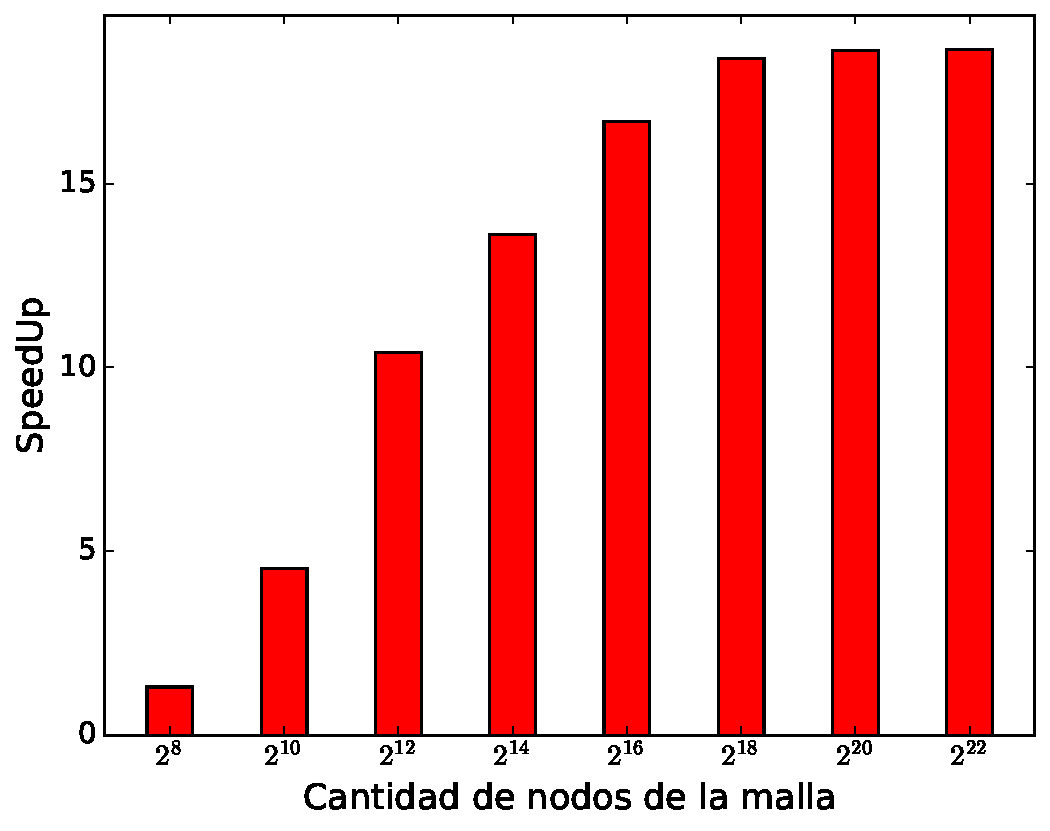
\includegraphics[width=0.75\textwidth]{Phoenix/LBCuda/lbcuda_760_simple}
	\caption{Speed Up realizado para el problema de construcci\'on de Maxwell en simple precisi\'on con una CPU Intel Core i7-3770 y GPU NVIDIA GeForce GTX 760.}
	\label{fig:lbcuda_760_simple}
\end{figure}

\begin{figure}[ht]
	\centering
	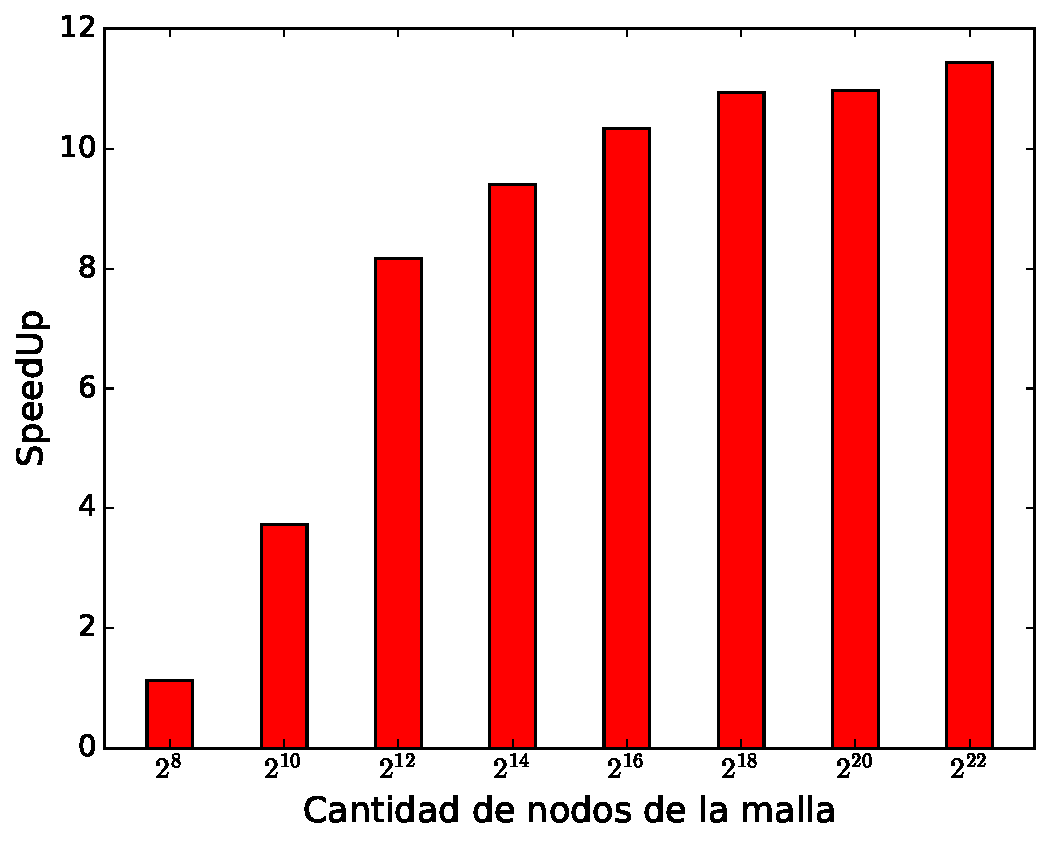
\includegraphics[width=0.75\textwidth]{Phoenix/LBCuda/lbcuda_760_doble}
	\caption{Speed Up realizado para el problema de construcci\'on de Maxwell en doble precisi\'on con una CPU Intel Core i7-3770 y GPU NVIDIA GeForce GTX 760.}
	\label{fig:lbcuda_760_doble}
\end{figure}
\FloatBarrier



\section{Listado completo de funcionalidades}

\subsection{Resolutores o \emph{solvers}}

\texttt{multiPhasePP}\: Flujo multif\'asico isot\'ermico mediante el m\'etodo pseudopotencial.
\medskip

\texttt{multiPhasePPHT}\: Flujo multif\'asico con transferencia de calor mediante el m\'etodo pseudopotencial.
\medskip

\texttt{multiPhasePPHT\_FD}\: Flujo multif\'asico con transferencia de calor mediante el m\'etodo pseudopotencial. La ecuaci\'on de energ\'ia se resuelve con esquemas de diferencias finitas.
\medskip

\texttt{vdWColumn}\: M\'odulo de Python para la resoluci\'on anal\'itica del problema de estratificaci\'on de un fluido vdW, cuyo algoritmo est\'a descripto en la \se{sec:vdw_1d}.
\medskip



\subsection{Generadores de malla}

\texttt{latticeBox2D}\: Grilla bidimensional rectangular, basada en conjuntos de velocidades D2Q$q$. Admite condiciones de contorno peri\'odicas.
\medskip

\texttt{latticeBox3D}\: Grilla tridimensional rectangular, basada en conjuntos de velocidades D3Q$q$. Admite condiciones de contorno peri\'odicas.
\medskip

\texttt{cartesianMesh}\: Grilla tridimensional con contornos escalonados, adaptada a una superficie en formato STL. 
\medskip

\texttt{salomesh}\: M\'odulo de Python para generaci\'on y exportaci\'on de mallas en SALOME, adaptando la grilla a un modelo CAD gen\'erico.
\medskip


\subsection{Fuerzas}

\texttt{adhesive}\: Fuerzas de adhesi\'on para modelos pseudopotencial.

\begin{itemize}
	\renewcommand{\labelitemi}{\hspace{2cm}}
	\setlength\itemsep{0.2em}
	\item \texttt{noAds}\: Sin fuerza de adhesi\'on
	\item \texttt{phiBasedMod}\: Fuerza de adhesi\'on en interfases l\'iquido-s\'olido, basada en un potencial modificado \cite{li_contact_2014}. Admite \emph{spots} de ancho variable, donde la magnitud de la fuerza puede ser uniforme o variar linealmente desde el centro. Estos \emph{spots} pueden ubicarse aleatoriamente sobre una superficie.
\end{itemize}
\medskip

\texttt{buoyant}\: Fuerza boyante. 

\begin{itemize}
	\renewcommand{\labelitemi}{\:}
	\item \texttt{fixedDensity}\: Constante, por ejemplo $\rho_{ref}g$.
	\item \texttt{averageDensity}\: Calculada en base a la densidad promedio.
\end{itemize}
\medskip

\texttt{external}\: Fuerza externa constante.
\medskip

\texttt{interaction}\: Fuerzas de interacci\'on

\begin{itemize}
	\renewcommand{\labelitemi}{\:}
	\item \texttt{singleRangeIntForce}\: Fuerza de interacci\'on considerando \'unicamente primeros vecinos (\eq{eq:f_int}).
	\item \texttt{singleRangeMixedIntForce}\: Fuerza de interacci\'on mixta, que surge de la combinaci\'on de esquemas de interacci\'on con primeros vecinos (\eq{eq:f_int_chen}).
	\item \texttt{singleRangeWithContact}\: Fuerza de interacci\'on con primeros vecinos. En una interfase l\'iquido-s\'olido estima los valores de densidad desconocidos mediante una aproximaci\'on geom\'etrica asociada a un \'angulo de contacto (\eq{eq:ding_angulo}).
	\item \texttt{singleRangeMixedWithContact}\: Fuerza de interacci\'on mixta con primeros vecinos. En una interfase l\'iquido-s\'olido estima los valores de densidad desconocidos mediante una aproximaci\'on geom\'etrica asociada a un \'angulo de contacto (\eq{eq:ding_angulo}).	
\end{itemize}
\medskip


\texttt{surfaceTension}\: T\'erminos adicionales para incluir efectos de tensi\'on superficial.

\begin{itemize}
	\renewcommand{\labelitemi}{\:}
	\item \texttt{noSurfaceTension}\: Sin t\'erminos adicionales.
	\item \texttt{liSutfaceTension}\: Modelo de tensi\'on superficial de Li.
	\item \texttt{liSutfaceTensionContact}\: Modelo de tensi\'on superficial de Li, estimando la densidad en interfases l\'iquido-s\'olido mediante la aproximaci\'on geom\'etrica para el \'angulo de contacto.
\end{itemize}



\subsection{Ecuaciones de estado}

\texttt{vanDerWaals}\: EOS de van der Waals.
\medskip

\texttt{CarnahanStarling}\: EOS de Carnahan-Starling.
\medskip

\texttt{PengRobinson}\: EOS de Peng-Robinson 
\medskip

\texttt{piecewiseLinear}\: EOS que considera una variaci\'on lineal de la presi\'on entre dos l\'imites de densidad. Uniforme fuera de los l\'imites.



\subsection{Fuentes de calor}

\texttt{noHS}\: Sin t\'ermino de fuente.
\medskip

\texttt{liHS}\: T\'ermino de fuente del modelo de Li para modelos pseudopotenciales. Conductividad t\'ermica constante.
\medskip

\texttt{markusHaziHS}\: T\'ermino de fuente del modelo de M\'arkus y H\'azi para modelos pseudopotenciales. Difusividad t\'ermica constante.



\subsection{Campos}

\texttt{scalarField}\: Campo escalar (por ejemplo $\rho$).
\medskip

\texttt{vectorField}\: Campo vectorial (por ejemplo $\bm{u}$).
\medskip

\texttt{pdfField}\: Funci\'on de distribuci\'on con $q$ componentes.



\subsection{Ecuaciones de LB}

\texttt{LiMRTEq}\: Modelo pseudopotencial de Li \cite{li_lattice_2013}.
\medskip

\texttt{XuMRTEq}\: Modelo pseudopotencial de Xu \cite{xu_three-dimensional_2015}.
\medskip

\texttt{GongSRTEq}\: Modelo SRT de Gong para ecuaci\'on de energ\'ia \cite{gong_lattice_2012}.
\medskip

\texttt{LiEnergyMRTEq}\: Modelo de Li para ecuaci\'on de energ\'ia \cite{li_improved_2017}.
\medskip

\texttt{myMRTEq}\: Modelo MRT para ecuaci\'on de energ\'ia presentado en los Cap\'itulos~\ref{chap:modelo2D} y \ref{chap:modelo3D}.



\subsection{Condiciones de contorno}

\texttt{ppNEBB}\: \emph{Bounce-back} de no equilibrio para modelos pseudopotenciales.
\medskip

\texttt{ppNEExt}\: Extrapolaci\'on de no equilibrio para modelos pseudopotenciales.
\medskip

\texttt{ppOutflow}\: Flujo saliente para modelos pseudopotenciales.
\medskip

\texttt{ppOutflowWithNEBB}\: Flujo saliente para modelos pseudopotenciales, con actualizaci\'on de la velocidad mediante extrapolaci\'on de no equilibrio.
\medskip

\texttt{ppPeriodic}\: condici\'on de contorno peri\'odica.
\medskip

\texttt{energyFixedCosT}\: Condici\'on de temperatura fija convariaci\'on cosenoidal. Incluye una perturbaci\'on sobre la distribuci\'on principal
\medskip

\texttt{energyFixedGradT}\: Gradiente de temperatura fijo.
\medskip

\texttt{energyFixedT}\: condici\'on de temperatura fija, basada en el esquema de Inamuro.
\medskip

\texttt{energyFixedTSpot}\: Gradiente de temperatura fijo, con \emph{spots} de diferente valor.
\medskip

\texttt{energyNormalHeatFlux}\: Condici\'on de flujo de calor fijo.
\medskip

\texttt{energyNormalHeatFluxSpot}\: Condici\'on de flujo de calor fijo, con \emph{spots} de diferente valor.
\medskip

\texttt{energyOutflow}\: Condici\'on de saloda para ecuaciones de energ\'ia.
\medskip

\texttt{energyPeriodic}\: Condici\'on de contorno peri\'odica.
\medskip

\texttt{NNExtFixedT}\: Condici\'on de temperatura fija en base a la extrapolaci\'on de no equilibrio.
\medskip

\texttt{NNExtFixedTSpot}\: Condici\'on de temperatura fija en base a la extrapolaci\'on de no equilibrio, con \emph{spots} de diferente valor.
\medskip



\subsection{Factores de relajaci\'on}

\texttt{uniformTau}\: Factores de ralajaci\'on uniformes y constantes en todo el dominio.
\medskip

\texttt{rhoPieceWise}\:  Factores de relajaci\'on constantes, que cambian a partir de un valor l\'imite de densidad.
\medskip

\texttt{rhoPieceWiseLinear}\: Factores de relajaci\'on que var\'ian linealmente, tomando dos valores de densidad l\'imite.
